\section{Background}
\label{sec:background_vocabs}

As established through the state of the art and in the comparative analysis performed in Sections \ref{sec:sota_vocabularies_analysis} and \ref{sec:sota_policies_analysis}, DPV contains the highest number of concepts to model GDPR's rights and obligations and their privacy terms, is being actively developed and maintained, is open and accessible, and ODRL supports the modelling of deontic concepts, e.g., permissions or obligations, constraints, e.g., spatial and temporal, and types of policies, e.g., offers, requests and agreements, and has a mechanism to develop extensions to its vocabulary through profiles.
As such, they can be used as a starting point to express policies for access to personal data, while invoking privacy and data protection-specific terms.

Figure \ref{fig:odrl} presents a diagram of the ODRL Information Model.
Its main goal is to \textit{``enable flexible Policy expressions by allowing the policy author to include as much, or as little, detail in the Policies''} \citep{iannella_odrl_2018}, using the terms defined in the ODRL Vocabulary \& Expression specification \citep{iannella_odrl_vocab_2018}.
Table \ref{tab:odrl} provides an overview of the concepts modelled in the ODRL vocabulary.

\begin{figure}[htbp]
\caption{ODRL Information Model, adapted from \cite{iannella_odrl_2018}.}
\label{fig:odrl}
\centering
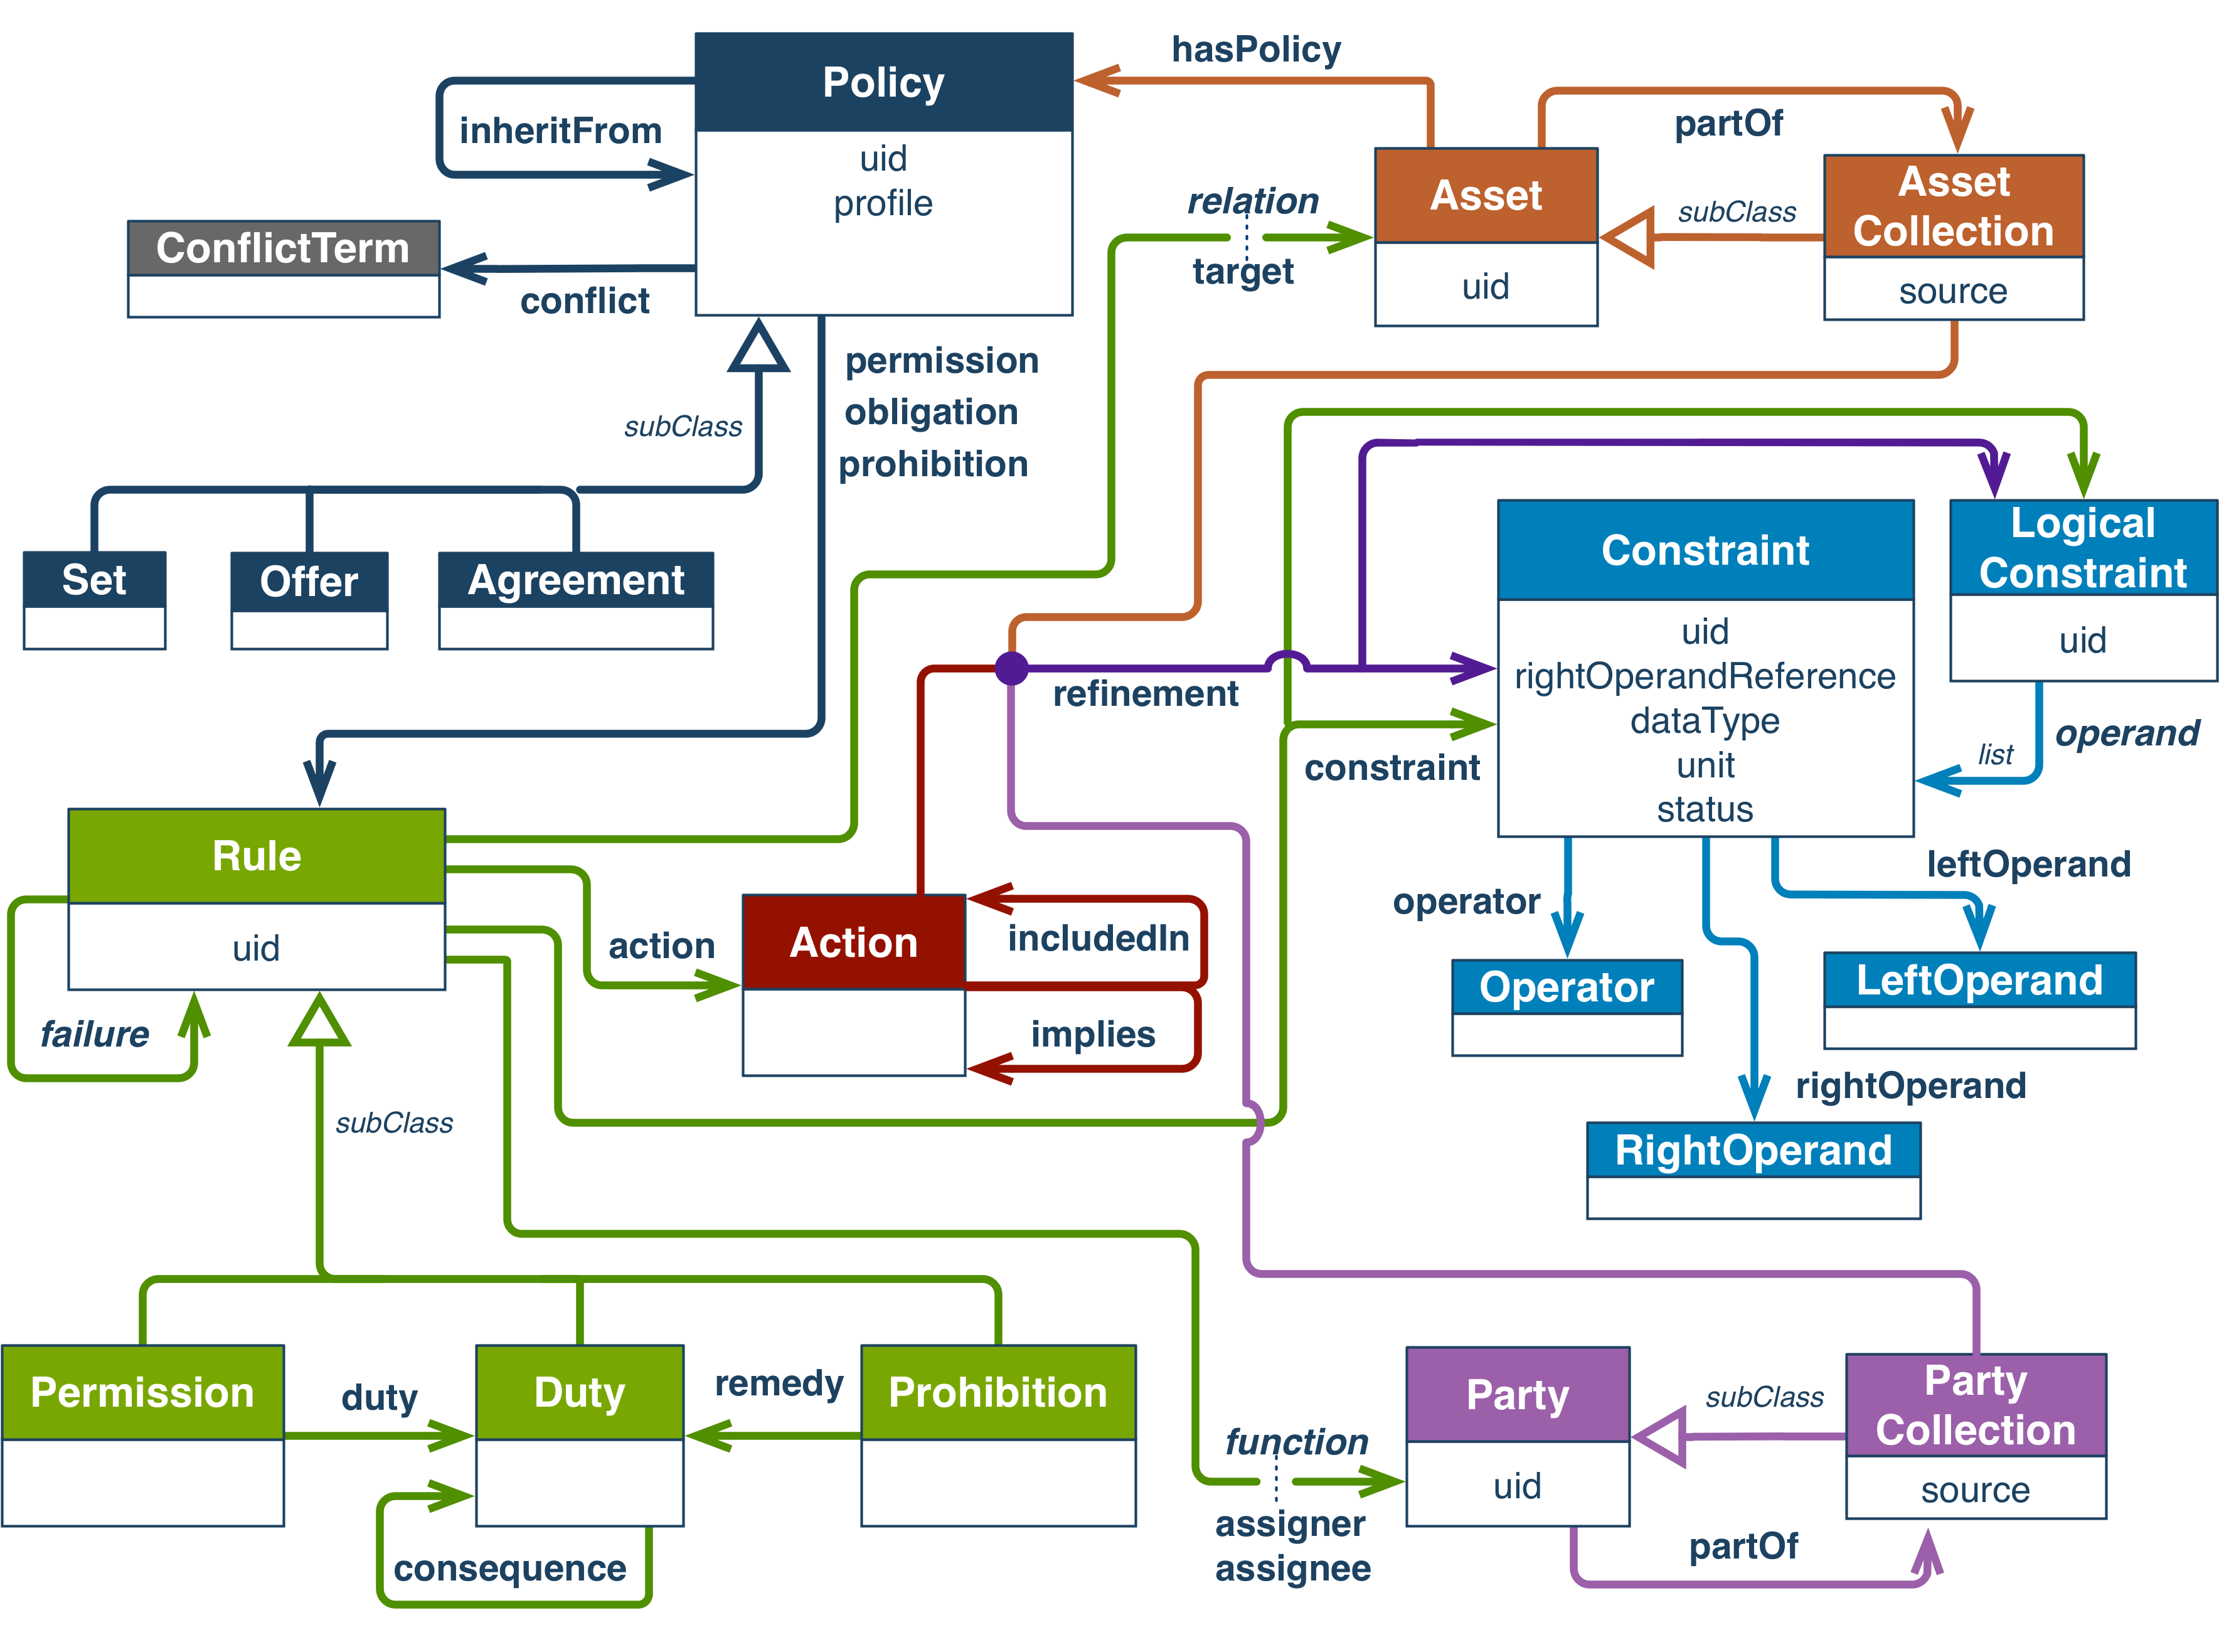
\includegraphics[width=0.8\textwidth]{figures/chapter-4/ODRL.png}
\end{figure}

\begin{table}[htbp]
\caption{Overview of the concepts modelled in the ODRL vocabulary.}
\label{tab:odrl}
\centering
\begin{tabular}{c||c}
Concept & Subclasses \\
\hline\hline
Policy & Agreement, Assertion, Offer, Privacy, Request, Set, Ticket \\
\hline
Rule & Duty, Permission, Prohibition\\
\hline
\begin{tabular}[c]{@{}c@{}}Party\\ functions\end{tabular} & \begin{tabular}[c]{@{}c@{}}assignee, assigner, attributedParty, attributingParty, \\ compensatedParty, compensatingParty, consentedParty, \\ consentingParty, contractedParty, contractingParty, informedParty, \\ informingParty, trackedParty, trackingParty\end{tabular}\\
\hline
Action & \begin{tabular}[c]{@{}c@{}}Attribution, CommericalUse, DerivativeWorks, Distribution, Notice, \\ Reproduction, ShareAlike, Sharing, SourceCode, acceptTracking, \\ aggregate, annotate, anonymize, archive, attribute, compensate, \\ concurrentUse, delete, derive, digitize, display, distribute, \\ ensureExclusivity, execute, extract, give, grantUse, include, index, \\ inform, install, modify, move, nextPolicy, obtainConsent, play, \\ present, print, read, reproduce, reviewPolicy, sell, shareAlike,\\ stream, synchronize, textToSpeech, transfer, transform, translate,\\ uninstall, use, watermark\end{tabular} \\
\hline
Operand & and, andSequence, or, xone \\
\hline
\begin{tabular}[c]{@{}c@{}}Left\\ Operand\end{tabular}    & \begin{tabular}[c]{@{}c@{}}absolutePosition, absoluteSize, absoluteSpatialPosition, \\ absoluteTemporalPosition, count, dateTime, delayPeriod, \\ deliveryChannel, elapsedTime, event, fileFormat, industry, \\ language, media, meteredTime, payAmount, percentage, product, \\ purpose, recipient, relativePosition, relativeSize, relativeSpatialPosition, \\ relativeTemporalPosition, resolution, spatial, spatialCoordinates, \\ systemDevice, timeInterval, unitOfCount, version, virtualLocation\end{tabular}\\
\hline
Operator & \begin{tabular}[c]{@{}c@{}}eq, gt, gteq, hasPart, isA, isAllOf, isAnyOf, isNoneOf, isPartOf,\\ lt, lteq, neq\end{tabular}\\
\hline
\begin{tabular}[c]{@{}c@{}}Right\\ Operand\end{tabular}   & policyUsage
\end{tabular}
\end{table}

The model also expresses which properties are mandatory and optional to define policies and their respective entities, assets, actions and constraints.
Both recommendations are being promoted and maintained by the W3C ODRL CG, which also aims to support the development of ODRL profiles and publish reports related to ODRL usage, such as:

\begin{itemize}
    \item the ODRL Implementation Best Practices \citep{smith_odrl_2023}, which presents examples of ODRL usage and describes good implementation practices;
    \item the ODRL Profile Best Practices \citep{steidl_odrl_2023}, which presents guidelines for the development, definition and publication of ODRL Profiles;
    \item the ODRL Formal Semantics \citep{fornara_odrl_2023}, which discusses and provides a formal semantics specification to ensure the correctness and consistency of services that use ODRL.
\end{itemize}

While ODRL presents itself as a well-tested resource for the expression of policies, it does contain the concepts to model personal data-related access policies or to invoke data protection-related terms.
As such, its profile mechanism provides an opportunity to extend the ODRL vocabulary with these missing terms, e.g., by associating it with personal data-focused vocabularies such as DPV.
Figure \ref{fig:dpv_base} provides an overview of DPV's core concepts.

\begin{figure}[htbp]
\caption{Overview of DPV's core concepts, adapted from \cite{pandit_primer_2022}.}
\label{fig:dpv_base}
\centering
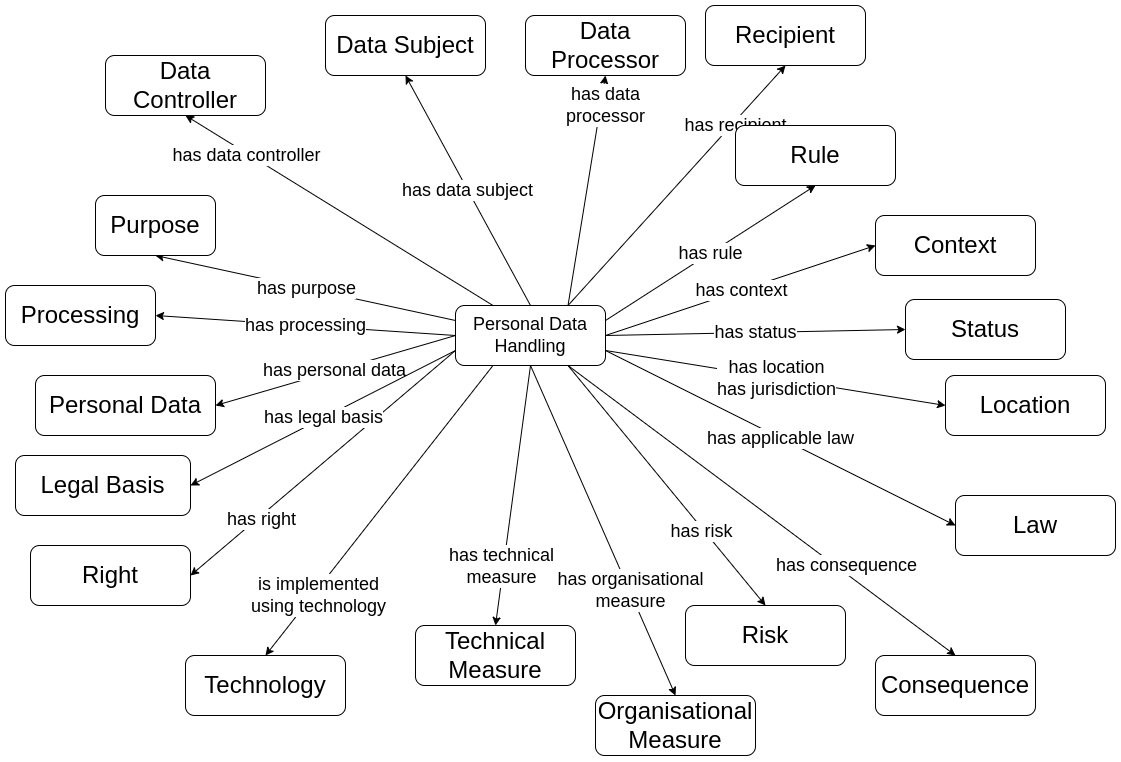
\includegraphics[width=0.8\textwidth]{figures/chapter-4/dpv-base.png}
\end{figure}

As indicated in the state of the art Chapter of this Thesis, DPV provides the most extensive list of data protection-related terms among the evaluated solutions.
Table \ref{tab:dpv_main_contributions} includes a list of the taxonomies defined in DPV's main specification, as well as the number of classes and properties defined in each taxonomy and, in the third column, the number of classes and properties that were contributed to the vocabulary in the course of the development of this Thesis.
These contributions were derived from the work developed and described throughout this Chapter, as well as Chapters~\ref{chap:matching} and~\ref{chap:dga}.

\begin{table}[htbp]
\centering
\caption[Taxonomies defined in DPV's main specification.]{Taxonomies defined in DPV's main specification, with the respective number of defined classes and properties, as well as the number of contributions of this Thesis to the vocabulary.}
\label{tab:dpv_main_contributions} 
\begin{tabular}{ c||c|c}
 Taxonomies & \#Classes (\#Properties)  & Contributions \\
 \hline\hline
 Entities & 4 (7) & 1 (4) \\
 \hline
 Legal Roles & 9 (9) & 0 (0) \\
 \hline
 Authorities & 5 (2) & 0 (0) \\
 \hline
 Organisations & 9 (0) & 0 (0) \\
 \hline
 Data Subjects & 26 (2) & 17 (0) \\
 \hline
 Purposes & 78 (2) & 20 (0) \\
 \hline
 Processing & 45 (1) & 0 (0) \\
 \hline
 Storage Conditions \& Automation & 29 (5) & 3 (0) \\
 \hline
 Scale of Processing & 27 (4) & 0 (0) \\
 \hline
 Data & 16 (2) & 0 (0) \\
 \hline
 TOMs & 139 (6) & 4 (0) \\
 \hline
 Legal Bases & 34 (5) & 0 (0) \\
 \hline
 Duration \& Frequency & 23 (11) & 7 (3) \\
 \hline
 Status & 39 (5) & 0 (0) \\
 \hline
 Location \& Jurisdiction & 25 (5) & 0 (0) \\
 \hline
 Risk \& Impacts & 16 (12) & 4 (3) \\
 \hline
 Rights & 9 (2) & 9 (0) \\
 \hline
 Rules & 4 (4) & 4 (4) \\
\end{tabular}
\end{table}

Moreover, the DPVCG also published a primer document~\citep{pandit_primer_2022}, which provides a description of DPV and its concept modelling, examples that illustrate how the provided concepts should be used to represent metadata regarding personal data handling activities and guidelines towards the application of DPV in particular use cases, e.g., consent record keeping or rights exercising.
Additionally, as previously described in Section~\ref{sec:dpv}, the DPVCG developed six extensions to the main specification, to model personal data categories, GDPR-specific concepts, technology and jurisdiction-relevant concepts, risk, and EU rights concepts.
Table~\ref{tab:dpv_extensions_contributions} includes a list of the DPV's extensions, as well as the number of classes and properties defined in each extension and, in the third column, the number of classes and properties that were contributed to the extensions in the course of the development of this Thesis.

\begin{table}[htbp]
\centering
\caption[DPV's extensions.]{DPV's extensions with the respective number of defined classes and properties, as well as the number of contributions of this Thesis to the extensions.}
\label{tab:dpv_extensions_contributions} 
\begin{tabular}{ c||c|c}
 Extensions & \#Classes (\#Properties)  & Contributions \\
 \hline\hline
 Personal data & 206 (0) & 3 (0) \\
 \hline
 GDPR & 92 (0) & 16 (0) \\
 \hline
 Technology & 60 (8) & 0 (0) \\
 \hline
 Jurisdiction & 452 (0) & 0 (0) \\
 \hline
 Risk & 376 (0) & 0 (0) \\
 \hline
 EU Rights & 62 (0) & 0 (0) \\
\end{tabular}
\end{table}

Additionally, existing work, using ODRL's profile mechanism, has been published to instantiate GDPR Articles as ODRL obligations~\citep{agarwal_legislative_2018} and as permissive, prohibitive or obligated policies with dispensations, which are translated into Answer Set Programming (ASP) rules for compliance checking~\citep{de_vos_odrl_2019}.
Other ODRL-based works have been published, related to (i) the representation of agreements to access data and execute algorithms in digital marketplaces~\citep{shakeri_modeling_2019}, (ii) the dynamic generation of privacy policies for IoT-generated data~\citep{canobenito_injecting_2023}, and (iii) the representation of privacy policies as ODRL requests, which use a small subset of DPV's taxonomies and do not follow the ODRL Information Model~\citep{krasnashchok_towards_2020}.